%
%   Data Clarification
%       - Plots...
%   
\clearpage
\section{Data clarification}
\label{section:data_clarify}

This section provides several visualizations to highlight the big pictures of our dataset, and it would
focus mostly on the behaviour of each variable as independent individuals, rather than the interaction 
between them, which we will focus in much details in \textbf{Section \ref{section:data_analysis}}.

\subsection{Categorical attributes}

\begin{figure}[H]
    \centering
    \begin{subfigure}[b]{0.49\textwidth}
        \centering
        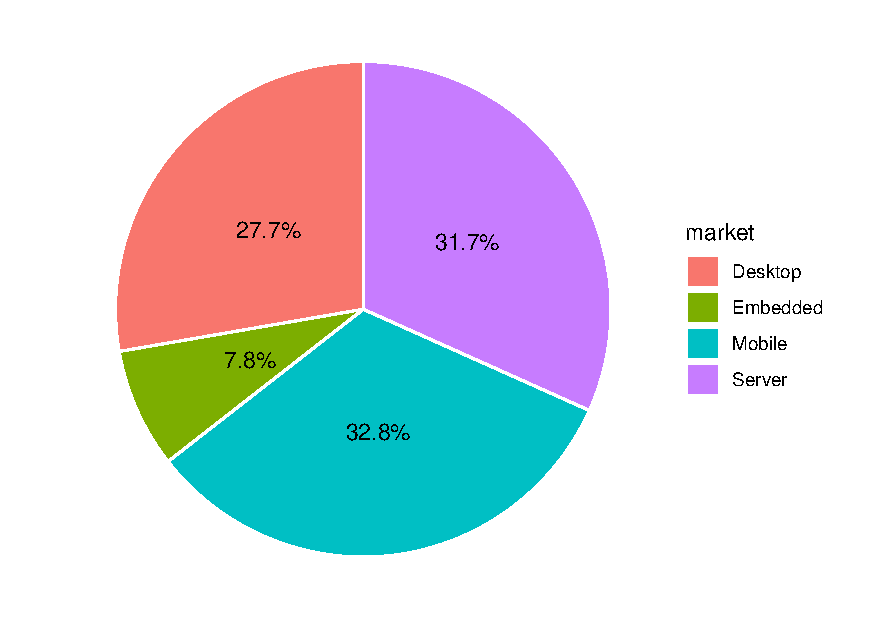
\includegraphics[width=\textwidth]{./graphics/pie_market.pdf}
        \caption{Pie of market share}
    \end{subfigure}
    \hfill
    \begin{subfigure}[b]{0.49\textwidth}
        \centering
        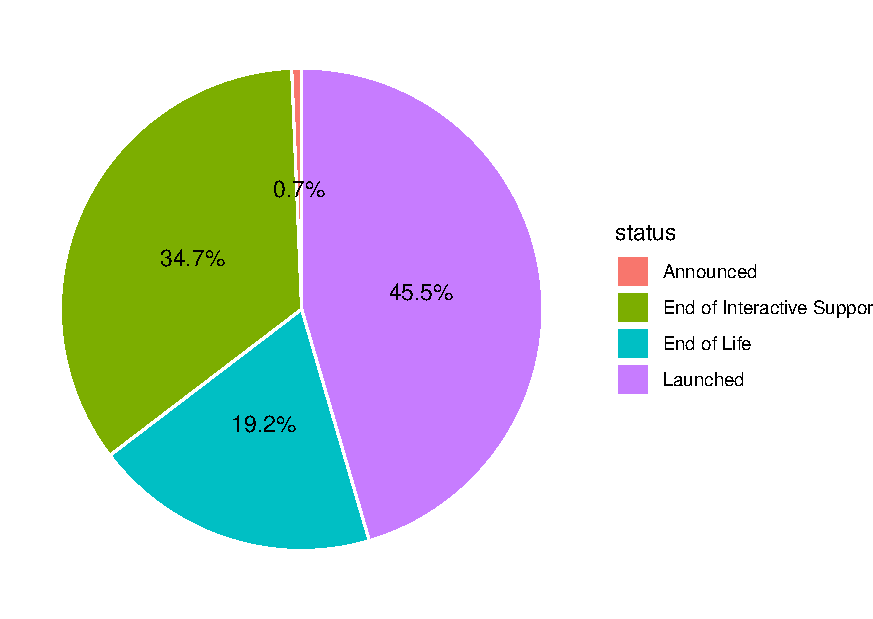
\includegraphics[width=\textwidth]{./graphics/pie_status.pdf}
        \caption{Pie of status}
    \end{subfigure}
    \caption{Pies of categorical attributes}
    \label{fig:pie_category}
\end{figure}

\inputcode[firstline=59,lastline=73]{R}{rcode/clarification.rmd}

\textbf{[Figure \ref{fig:pie_category}]} Two obvious categorical attributes of our data are \textit{Market} and \textit{Status}.
\begin{itemize}
    \item In \textit{Market} attribute, three primary shares of market are Desktop, Server and Mobile. Embedded constitues a very small
    proportion.
    \item In \textit{Status} attribute, most of them are Launched, End of Life or End of interactive support. A tiny amount of Announce
    contributes modestly to total amount of CPU's model by provider Intel.
\end{itemize}

In terms of the code we used to plot two above pies. Each line is self-explanatory. Since two pies have different configurations, and would be
verbose to explain everything here, we leave the detailed implementation in \verb|rcode/clarification.rmd|. A few things to note are:
\begin{itemize}
    \item \verb|data_percentages| is a data-frame containing three properties: \verb|market|, \verb|value| and \verb|percent|.
    Note that, we use variable \verb|market| two times: one for plotting market-pie and one for plotting status-pie. This is just for ease
    of use and avoid repeating the code. It should not be taken seriously (the same name for two different things could be confusing).
    \item \verb|market| are the levels of \verb|market|-attribute (or \verb|status|-attribute)
    \item \verb|value| is the vector of frequencies of each \verb|market| (or \verb|status|)
    \item \verb|percent| is the vector percentages (computed by dividing the frequency by total and multiply by $100$)
\end{itemize}





\subsection{Continuous attributes}

\begin{figure}[H]
    \centering
    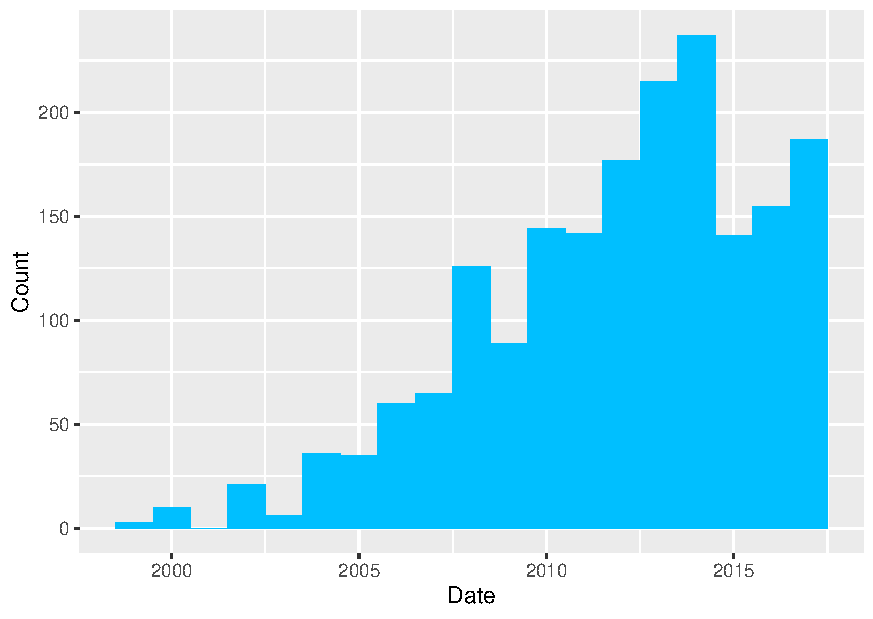
\includegraphics[width=0.5\textwidth]{./graphics/hist_ldate.pdf}
    \caption{Histogram of launch date}
    \label{fig:hist_ldate}
\end{figure}

\inputcode[firstline=78,lastline=80]{R}{rcode/clarification.rmd}

\textbf{[Figure \ref{fig:hist_ldate}]} The \textit{Launch date} histogram shown that most of Intel's CPUs are launched recently, 
with two notable peaks at 2014 and 2017. This would affect tremendously to the bias of the data since some variables are dependent 
on \textit{Launch date}, making the prediction models (\textbf{Section \ref{section:data_analysis}}) weight the recent CPUs heavily,
instead of old, legacy CPUs which are also neccessary to capture a fair pattern over the time.






\begin{figure}[H]
    \centering
    \begin{subfigure}[b]{0.49\textwidth}
        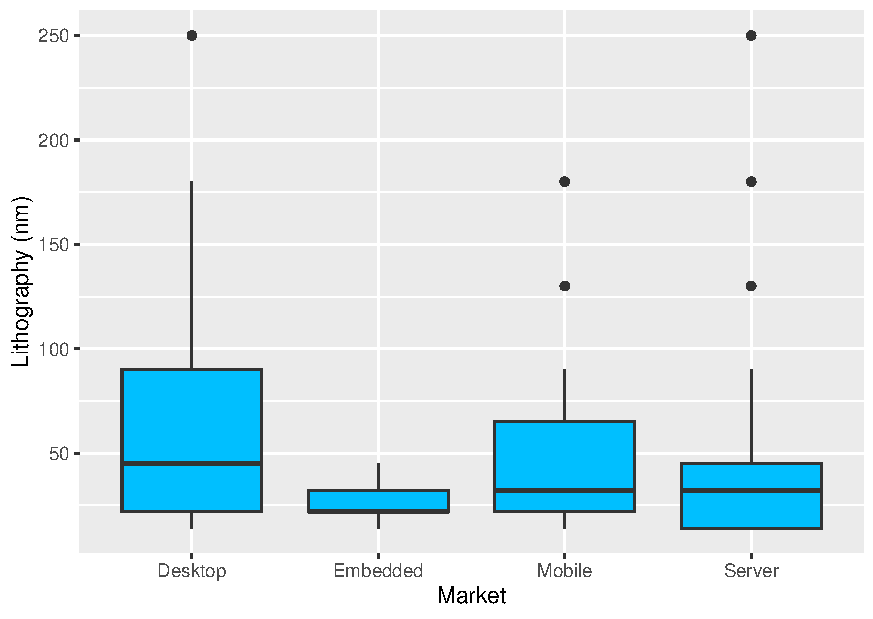
\includegraphics[width=\textwidth]{./graphics/box_litho.pdf}
        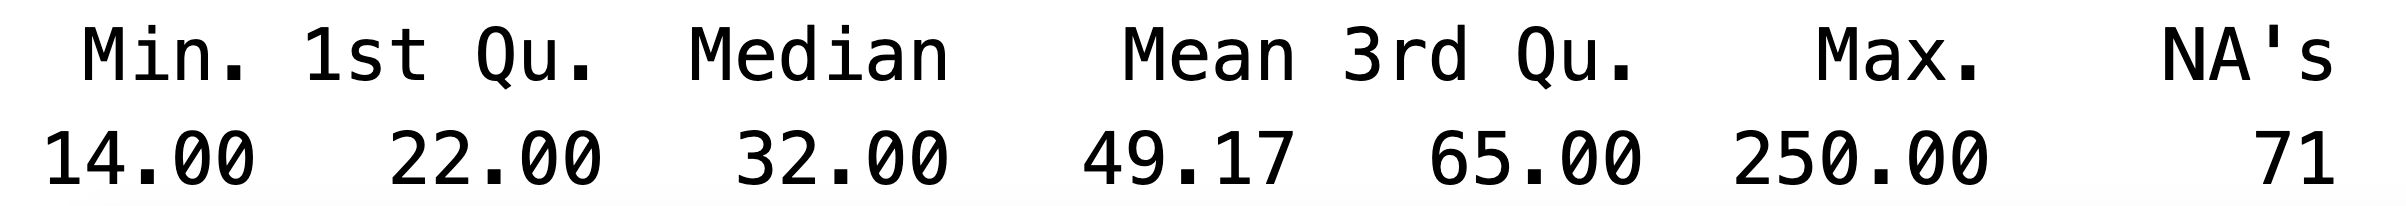
\includegraphics[width=\textwidth]{./graphics/sum_litho.png}
        \caption{Box plots and Summary of Lithography}
        \label{fig:box_litho}
    \end{subfigure}
    \hfill
    \begin{subfigure}[b]{0.49\textwidth}
        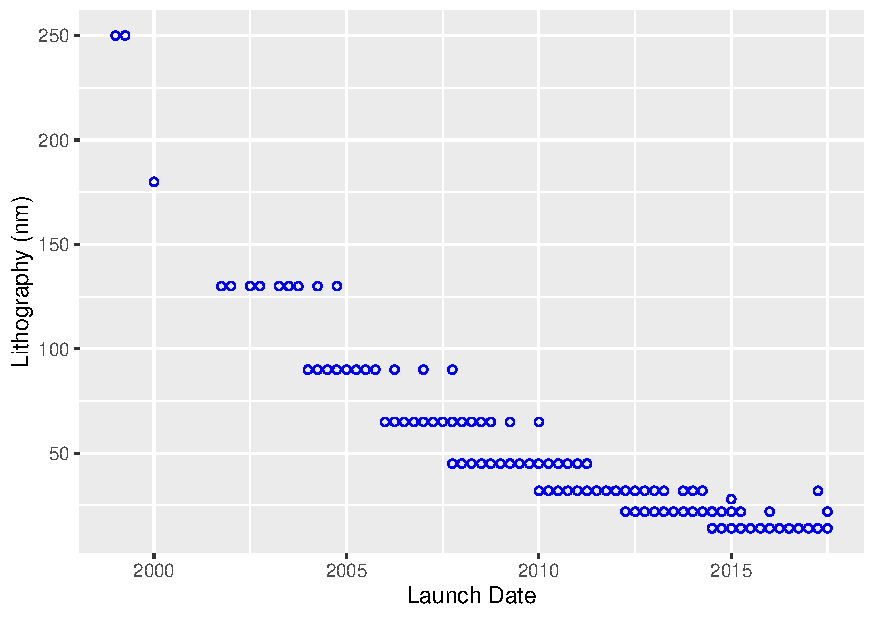
\includegraphics[width=\textwidth]{./graphics/scatter_litho.pdf}
        \caption{Plot of lithography over time.}
        \label{fig:scatter_litho}
    \end{subfigure}
    \caption{Lithography plots}
\end{figure}

\inputcode[firstline=85,lastline=89]{R}{rcode/clarification.rmd}

\inputcode[firstline=94,lastline=96]{R}{rcode/clarification.rmd}

\textbf{[Figure \ref{fig:box_litho}]} The box plot of \textit{Lithography} (chip printing technique) demonstrates interesting characteristics:
\begin{itemize}
    \item There was a large variance in the types of Lithography designed in Intel's Desktop processors, a smaller, but significant variance of 
    Mobile and Server are also observed. Embedded is less diverse, however, and also concentrates mostly on small \textit{Lithography} printings.

    \item The mean of \textit{Lithography}, in whatever market, is also approximately the same. That number might represents the most suitable 
    printing technique that is widely used among Intel's CPUs.
\end{itemize}

Overall, the most common \textit{Lithography} is $32 nm$. The best printing technique possible was $14 nm$ and the worst was $250 nm$. That large
number might come from old, legacy processors which were not designed with recent innovations in the Chip industry.

\textbf{[Figure \ref{fig:scatter_litho}]} The scatter plot of \textit{Lithography} with respect to \textit{Launch date} shown that the lithography
is getting smaller over time, and they are categorized into specific time intervals. The fact the \textit{Lithography} spans the distribution over
an interval of time instead of condensed into a specific quarter like \textit{Launch date} make it more powerful than \textit{Launch date}. In our
models, we always use \textit{Lithography} instead of \textit{Launch date}. This fact will be visualized with numbers later to make this argument 
more convincing.







\begin{figure}[H]
    \centering
    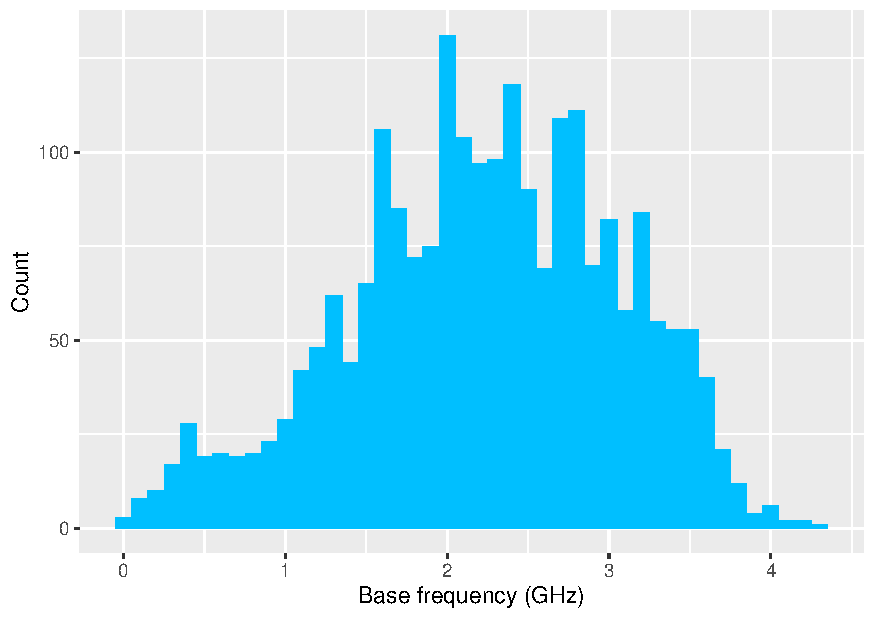
\includegraphics[width=0.5\textwidth]{./graphics/hist_bfreq.pdf}
    \caption{Histogram of Base Frequency}
    \label{fig:hist_bfreq}
\end{figure}

\inputcode[firstline=108,lastline=110]{R}{rcode/clarification.rmd}

\textbf{[Figure \ref{fig:hist_bfreq}]} The most significant trend that could be observed in the \textit{Base frequency} histogram is its "normality".
It can be seen that, the shape of \textit{Base frequency} disribution is convincingly a bell, and most \textit{Base frequency} concentrates around
the mean (around $2.3$ GHz). This is expected since high \textit{Base frequency} can influence the amound of heat a CPU produces, and there are always
trade-offs between performance and heat. This relationship (between heat and performance) will be visualized in \textbf{Section \ref{section:data_analysis}}.






\begin{figure}[H]
    \centering
    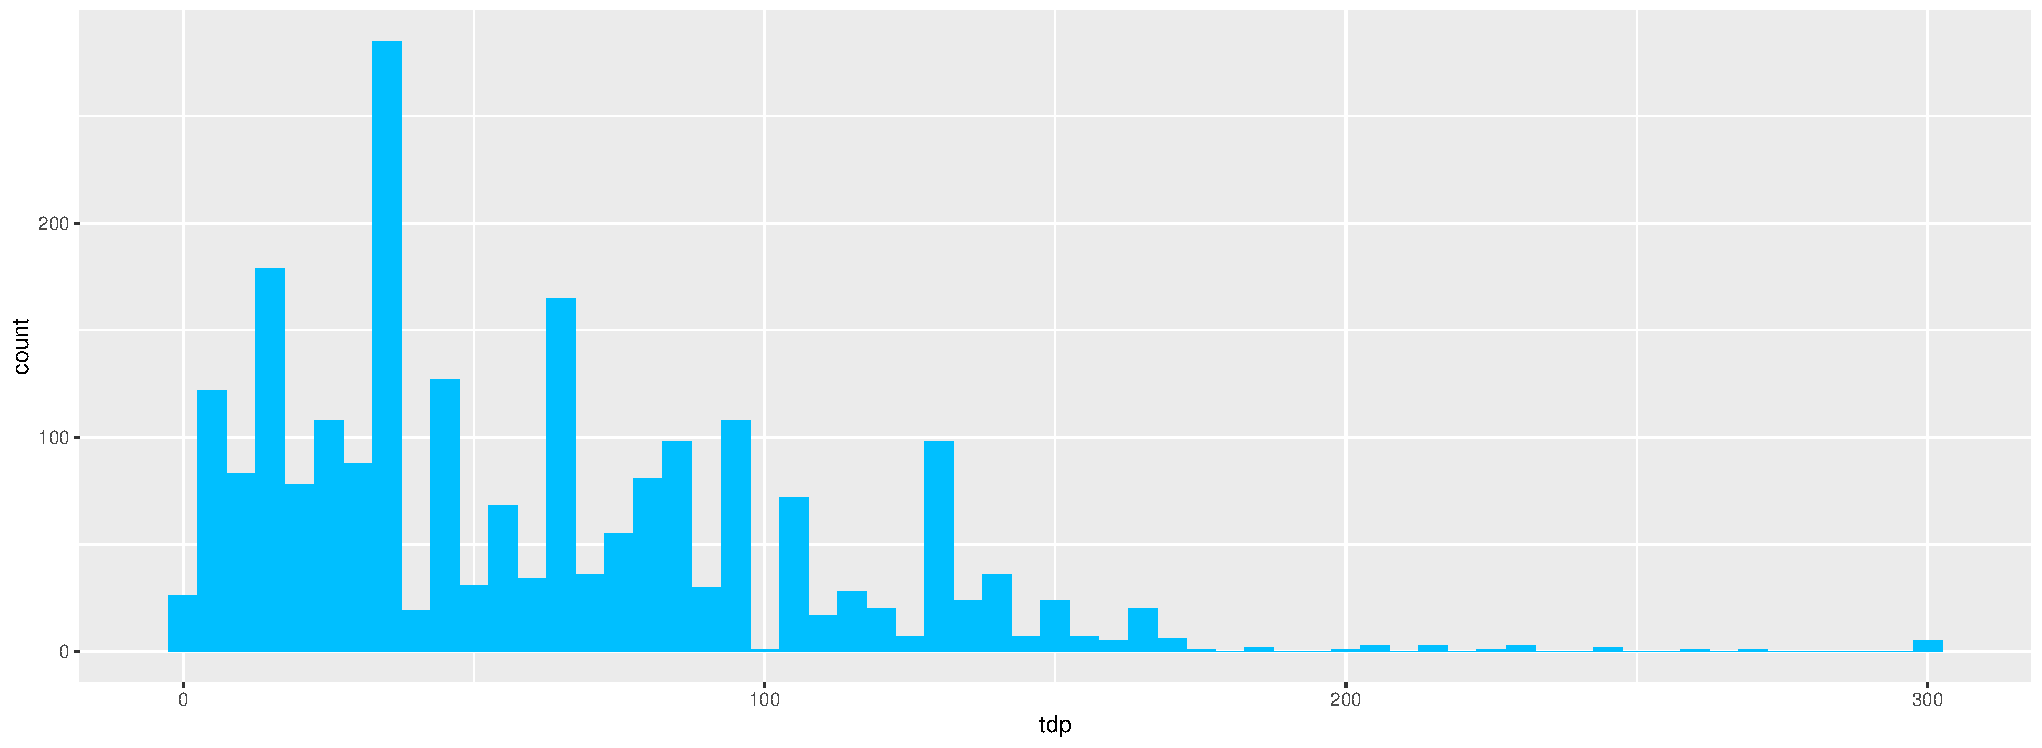
\includegraphics[width=0.5\textwidth]{./graphics/hist_tdp.pdf}
    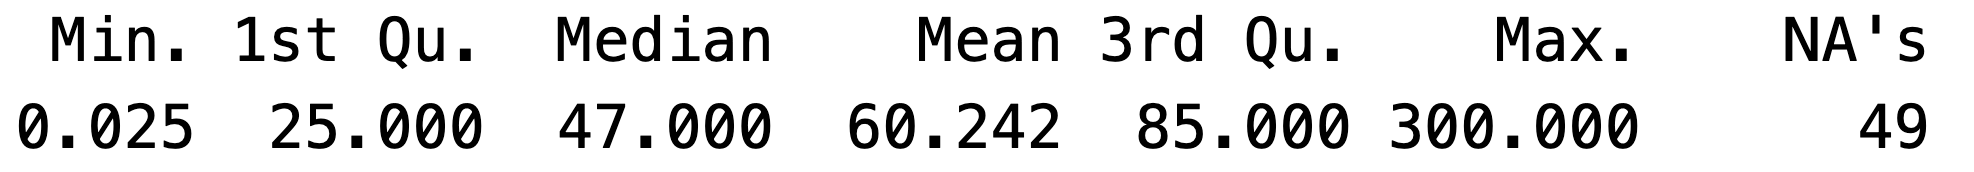
\includegraphics[width=0.5\textwidth]{./graphics/sum_tdp.png}
    \caption{Box plots and Summary of Thermal Design Power}
    \label{fig:hist_tdp}
\end{figure}

\inputcode[firstline=115,lastline=119]{R}{rcode/clarification.rmd}

\textbf{[Figure \ref{fig:hist_tdp}]} \textit{Thermal design power} is the of main interest in our topic. We can see that, the distribution of \verb|TDP| varies
wildly, from 0W to 300W. However, the occurences of values $\ge 150$W is rare (we can see the 75\%-quantile is at 85W), indicating that we can treat these values 
as outliners and remove them before carrying further analysis.